Informatyka i jej wszystkie dziedziny pokrewne bez możliwości wizualizacji nie byłyby tym, czym są dzisiaj. Bez rozwoju grafiki komputerowej zakres, w jakim można wykorzystywać komputery, byłby dużo mniejszy - nie istniałyby gry komputerowe, filmy pozbawiono by efektów specjalnych (aspekty artystyczne), a brak możliwości graficznej wizualizacji badań i projektów ograniczyłby rozwój technologiczny. Dlatego też metody generowania obrazów są nie tylko nieustannie doskonalone, ale i stały się przedmiotem badań licznej grupy specjalistów. Jedną z pierwszych metod pozwalających na renderowanie fotorealistycznych grafik jest tzw. \emph{metoda śledzenia promieni} (ang. \emph{ray tracing}. Jej początki zawdzięczamy Arthur'owi Appel'owi oraz Robert'owi Goldstein'owi i Roger'owi Nagel'owi, natomiast rekursywny algorytm po raz pierwszy wprowadził Turner Whitted - jego rozwiązanie uwzględniało również promienie odbite od powierzchni i takie, które uległy załamaniu.

\begin{figure}[H]
\centering
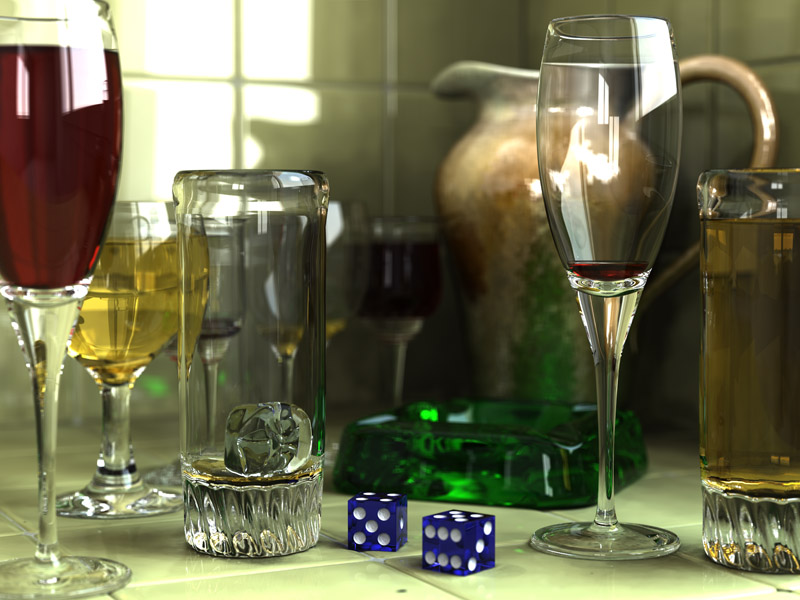
\includegraphics[width=14cm]{glasses.jpg}
\caption{Glasses - grafika wygenerowana przy użycie programy \emph{POV-Ray}, autor: Gilles Tran, źródło: http://www.oyonale.com/modeles.php?lang=en\&page=40}
\end{figure}

Metoda śledzenia promieni jest stosunkowo prostym algorytmem, który pozwala na generowanie bardzo złożonych i realistycznych grafik uwzględniających wiele zjawisk fizycznych. Wadą takiego rozwiązanie jest bardzo długi czas generowania obrazu, dlatego nie jest ono wykorzystywane w aplikacjach interaktywnych. Zamiast tego wykorzystuje się tzw. \emph{computer graphics pipeline} - skomplikowaną, wspieraną sprzętowo sekwencję kroków wykorzystywanych w bibliotekach graficznych takich jak \emph{OpenGL} (dokładny opis działania można znaleźć w \cite{gpipe}). Pozwala ona na szybkie renderowanie obiektów, jednak obrazy wygenerowane tą metodą nie będą już tak realistyczne - wiele pracy wkłada się w poprawienie ich jakości.

Podstawowym pytaniem, jakie jest stawiane w tej pracy, jest to, czy metoda śledzenia promieni ma szansę być wykorzystywana w aplikacjach interaktywnych tak, aby obliczenia związane z generowaniem obrazu były niewidoczne dla użytkownika? Jakie parametry sceny pozwalają na generowanie obrazu z zadowalającą prędkością? Czy zrównoleglenie obliczeń pozwoli zbliżyć się do minimalnego progu 24 klatek na sekundę tak, aby można było mówić o generowaniu obrazu w czasie rzeczywistym? W jaki sposób moglibyśmy przyspieszyć obliczenia?  Wiele z tych pytań pozostanie otwartych, jednak badania takie jak te są próbą znalezienia na nie odpowiedzi.


\section{Wykazu celów i zadań pracy}

Celem niniejszej pracy jest:
\begin{enumerate}
\item Dokonanie analizy problemu na podstawie zebranej literatury.
\item Określenie wymagań jakie powinien spełniać system.
\item Dobór narzędzi programistycznych w celu zaimplementowania systemu realizującego algorytm śledzenia promieni.
\item Zaprojektowanie systemu.
\item Implementacja systemu.
\item Przeprowadzenie badań nad algorytmem metody śledzenia promieni.
\item Omówienie rezultatów.
\item Zaproponowanie dodatkowych rozwiązań mających na celu przyspieszenie obliczeń.
\end{enumerate}

\section{Budowa pracy}

Niniejszy dokument składa się z ośmiu rozdziałów - ten, stanowiący wstęp, jest jednym z nich. W rozdziale drugim znajduje się dogłębna analiza problemu - zostały tam w sposób szczegółowy przedstawione wszystkie podejmowane zagadnienia. W rozdziale trzecim zostały zaproponowane technologie, które pozwolą na implementację programu mającego realizować rekursywną metodę śledzenia promieni z wykorzystaniem obliczeń równoległych. Na początku rozdziału czwartego zostały zdefiniowane wymagania i założenia, jakie powinien realizować program. Kolejne podrozdziały w sposób bardziej formalny i szczegółowy pokazują architekturę aplikacji. W rozdziale piątym zostały zawarte niektóre szczegóły implementacyjne gotowego już programu. Rozdział szósty opisuje, w jaki sposób program działa - przedstawiono tam podstawową instrukcję jego obsługi oraz budowę pliku wejściowego. Rozdział siódmy zawiera rezultaty przeprowadzonych testów, wraz z ich omówieniem. Znajdują tam się również przykładowe obrazy, jakie zostały wygenerowane przez działającą aplikację. W rozdziale ósmym znajduje się podsumowanie pracy wraz z propozycjami kierunku dalszych badań.